% VUT FIT MITAI
% MSZ 2021/2022
% Author: Vladimir Dusek
% Login: xdusek27

%%%%%%%%%%%%%%%%%%%%%%%%%%%%%%%%%%%%%%%%%%%%%%%%%%%%%%%%%%%%%%%%%%%%%%%%%%%%%%%%

% Path to figures
\graphicspath{{prl/klasifikace_paralelnich_architektur/figures}}

%%%%%%%%%%%%%%%%%%%%%%%%%%%%%%%%%%%%%%%%%%%%%%%%%%%%%%%%%%%%%%%%%%%%%%%%%%%%%%%%

\chapter{PRL~--~Klasifikace a vlastnosti paralelních a distribuovaných architektur, základní typy jejich topologií.}

%%%%%%%%%%%%%%%%%%%%%%%%%%%%%%%%%%%%%%%%%%%%%%%%%%%%%%%%%%%%%%%%%%%%%%%%%%%%%%%%

\section{Zdroje}

\begin{compactitem}
    \item \path{PRL_01_02_Arch_MNG.pdf}
    \item \textit{Otázka není vysázená, pouze vloženo exportované PDF z google docs.}
\end{compactitem}

%%%%%%%%%%%%%%%%%%%%%%%%%%%%%%%%%%%%%%%%%%%%%%%%%%%%%%%%%%%%%%%%%%%%%%%%%%%%%%%%

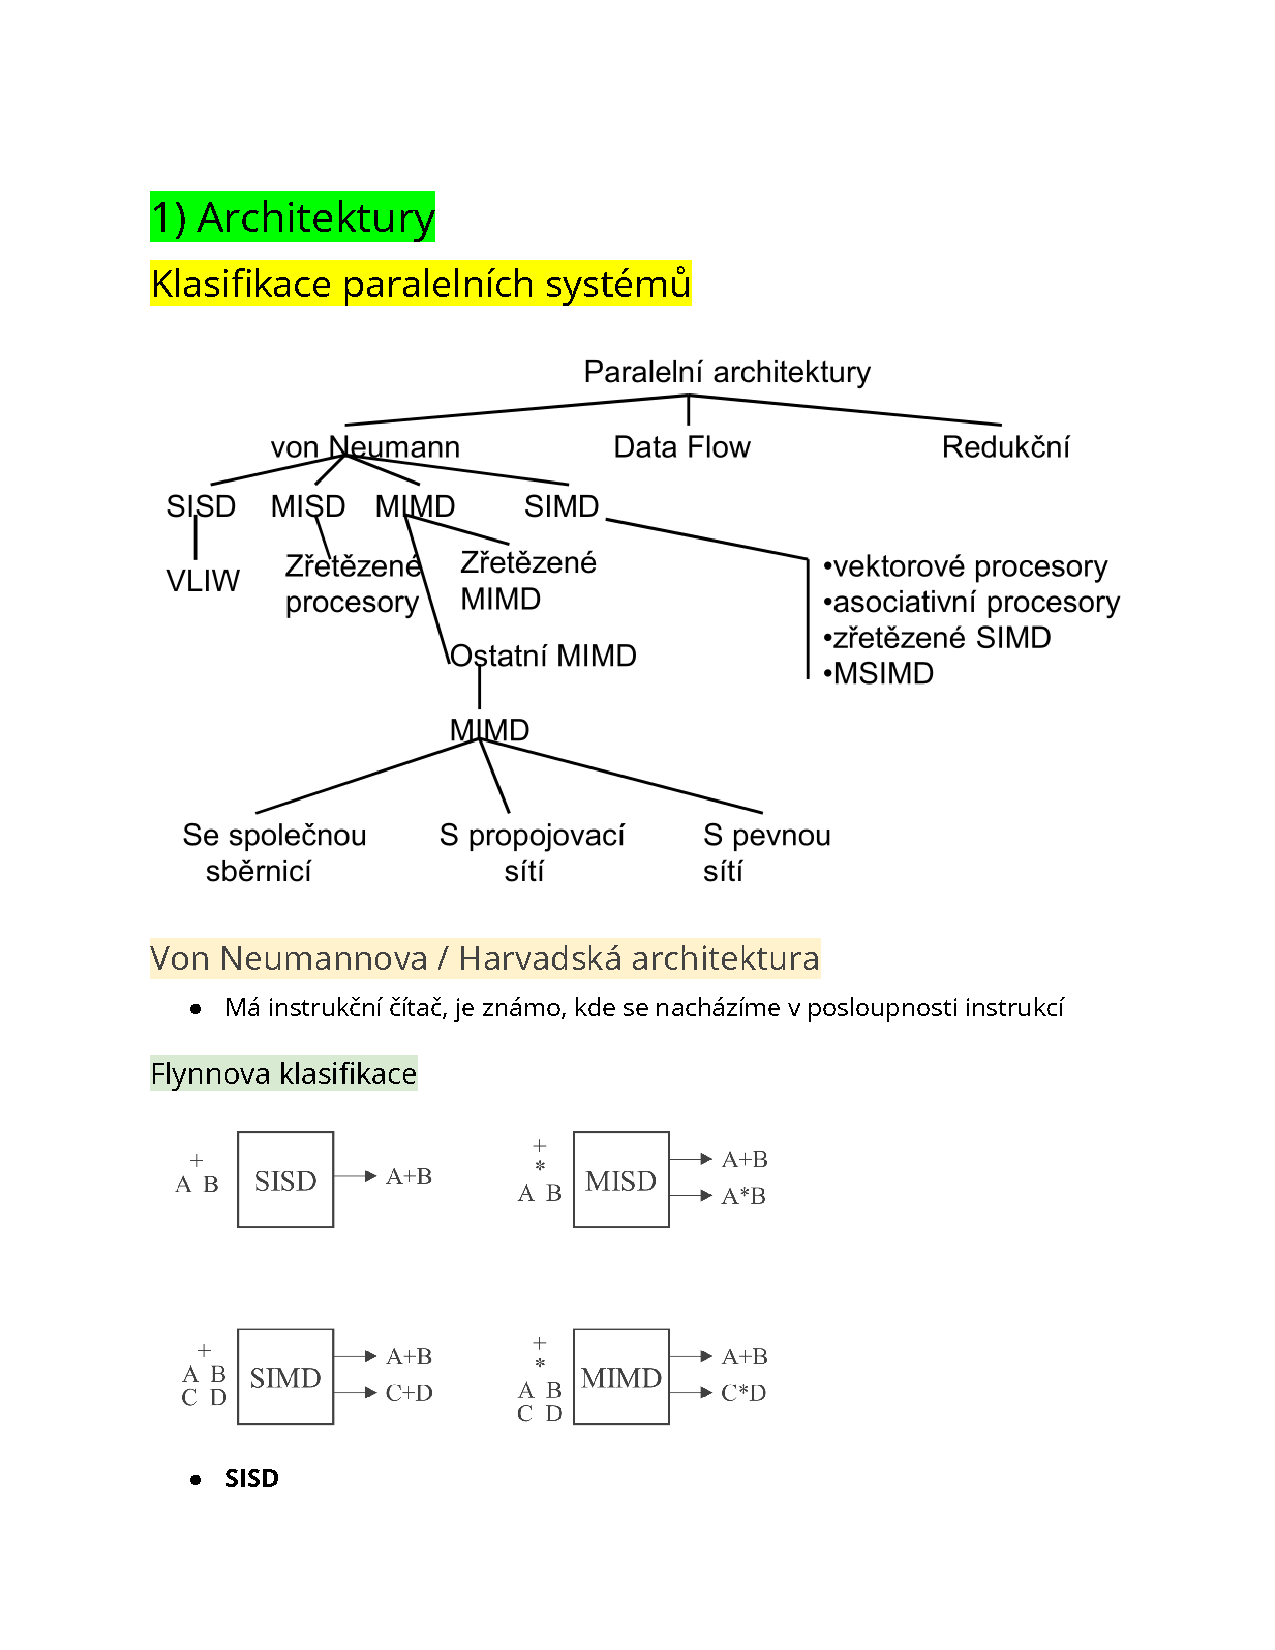
\includepdf[pages=-]{prl/klasifikace_paralelnich_architektur/gdocs_prl_1_2.pdf}
